%!TeX spellcheck = en_GB
\documentclass[conference]{IEEEtran}
\IEEEoverridecommandlockouts
\usepackage{cite}
\usepackage{amsmath,amssymb,amsfonts}
\usepackage{algorithmic}
\usepackage{graphicx}
\usepackage{textcomp}
\usepackage{xcolor}

\begin{document}
	
	% describe the protocol for control access (blockchain part)
	%  Related work
	%	-   traditional architectures commenly employed in the IoT access:
	%	   XACML, OAuth, UMA
	%	   Dependency of a central entity

\title{Distributed Authorized Medical Data Management}
%\title{Distributed Authorized Medical Data Updates}
%\title{Authorized Updates to Distributed Medical Data}

% We talk more about updates, shall we just use updates on title?

\author{
	\IEEEauthorblockN{%
		Chunmiao Li\textsuperscript{1,3},
		Yang Cao\textsuperscript{2},
		Zhenjiang Hu\textsuperscript{1,3,4},
		Masatoshi Yoshikawa\textsuperscript{2}
	\vspace{1.5ex}
	\IEEEauthorblockA{%
		\textsuperscript{1}\,National Institute of Informatics, Japan\qquad
		\textsuperscript{2}\,Kyoto University, Japan \\
		\textsuperscript{3}\,SOKENDAI (The Graduate University for Advanced Studies), Japan\qquad
		\textsuperscript{4}\,University of Tokyo, Japan
	}
%	\vspace{1ex}
%	\IEEEauthorblockA{%
%		Email:\
%		\textsuperscript{1}\,chunmiaoli1993@nii.ac.jp,
%		\textsuperscript{2}\,yang@i.kyoto-u.ac.jp,
%		\textsuperscript{3}\,hu@nii.ac.jp,
%		\textsuperscript{4}\,yoshikawa@i.kyoto-u.ac.jp
%	}
}
}

\maketitle

%regulate the use of a, an, the
\begin{abstract}
	Electronic Medical data sharing between stakeholders, such as patients, doctors and researchers, can promote more effective medical treatment collaboratively. These sensitive and private data could only be accessed by authorized users.  Given a total medical data, users may care parts of them and other unrelated information might interfere the user-interested data search and increase the risk of exposure. Besides accessing these data, users may want to update them and propagate to other sharing peers so that all peers keep identical data after each update. To satisfy these requirements, in this paper we propose a medical data sharing architecture that addresses the permission control using smart contracts on blockchain and splits data into pieces shared with different peers then synchronize complete data and these pieces after updates with bidirectional transformations. Medical data reside on each user's local database and permission-related data are stored on smart contracts. Only all peers have gained the newest shared data after updates can they start to do next operations on it, which are enforced by smart contracts. Blockchain-based  immutable shared ledge enable users to trace data updates history. This paper can provide a new perspective to view complete medical data as different slices to be shared with various peers but consistency after updates between them are still promised, which can protect privacy and improve data search efficiency.

\end{abstract}

\begin{IEEEkeywords}
medical data, authorization, update, distributed
\end{IEEEkeywords}

\section{Introduction}

Now a lot of medical data are digitalized so as to be stored and accessed conveniently. A medical record is produced after a patient go to see doctor and often resides on the hospital's database. Medical records contain highly sensitive information about patient privacy. HIPPA Privacy Rule  \cite{centers2004hipaa} in the U.S. regulates the use and disclosure of personally identifiable health information to protect patients' privacy. However, it hard to make sure that all medical institutes would follow these rules and they may expose patient privacy deliberately or for profit. Moreover, a patient might visit many hospitals and leave his records scattered \cite{zhang2016secure} in different places, which make it hard for him to manage his records efficiently. So patient should be provided a platform to manage and review his historical medical data in case of exposure or being tampered. What's more, better communication between patients and doctors can contribute to patient adherence \cite{zolnierek2009physician} and  improved health \cite{street2009does}. In addition to provide data to doctor, patients tend to share their medical data with health experts to help understand some complex statistics. Many researches has been done to study how medical specialists with different expertise collaborate with each other \cite{fitzpatrick2013review}.  Researchers can identify public hearth risks and then develop a better treatments by analyzing existing medical data \cite{office2015report}. As presented in \cite{chung2018using},  patients and experts can exchange information to develop better plans to satisfy individual routines. Sharing medical data under some constraints could benefit all relating stakeholders such as patients, researchers and doctors. 
% %patient understand and trace his medical records
% %doctor revise treatment plan in terms of feedback
% %researcher conduct census analyzation and provide better measures

To be shared by multiple parties, medical data could reside in encrypted formats on a trusted cloud storage server. Only authorized stakeholders can access the shared data. Centralized access control might lead to single point of failure and become the bottleneck of sharing system. Some medical data sharing systems \cite{azaria2016medrec,fan2018medblock,xia2017bbds} are proposed to manage authentication based on blockchain\cite{nakamoto2008bitcoin} technology. Being a immutable shared ledger, blockchain can achieve consensus among distributed nodes via proof of work. Encoding the access control logic of medical data into smart contracts\cite{azaria2016medrec} or Chaincode \cite{dubovitskaya2017secure} can prevent unauthorized party to access medical data, which will guarantee data security. Anyone who want to access medical data should be verified permission from blockchain side and their access process will be recorded on blockchain.

We identified that there are still other requirements on data sharing and ignored by current works. 

Firstly, generally different stakeholders may have different focus on the same medical records. For example, doctors might be more concerned with the clinical data and researchers are interested in mechanism of action, whereas patients care more about the medicine dosage standard. Moreover, doctors may add some terminologies on records which might put patients in confusion and fear. Also, some statistics about hospital internal facilities should not be exposed to patients for privacy protection.  To reduce the size of shared data to improve access efficiency and avoid additional data interference, the complete medical data (data source) might be split into lots of smaller data pieces (data views) which are shared by different peers. Each view can be regenerated from the source. Source and view should satisfy predefined consistency relationship. Different views from one source might have overlapped data. Moreover, each party will have a local complete data and different data pieces to share with others. In this way, shared data are distributed among sharing parties.

Secondly, not only limited to access data, patients or doctors may want to update existing shared data. Although some works \cite{azaria2016medrec} claimed to allow updates on shared medical data, they did not propose any concrete scheme to implement updates and details about how to synchronize all sharing peers to keep them still have same shared data after updates.

%read, add, delete shared data belong to data management.
%Since the shared data just reside in each peer's local database, read the shared data is easily promised.
In this paper, we aim to solve these two issues on distributed shared medical data as stated above. 
%for updates distributed shared medical data
Each participant may have multiple shared data\footnote{Our work assume that the initialization of shared data has been finished. We only consider management on existing shared data.} with different peers and keep this shared ones consistent with complete medical records. We apply bidirectional transformations \cite{hu2014validity} to synchronize them after updates on either one side. For example, we can invoke \emph{put} direction of a  BX program to reflect modifications on shared data to complete data and \emph{get} to reproduce shared data from complete data. 
%For authorization
Moreover,  any operations on the shared data should be conducted after the peer has been authorized. Permission related data are encoded into smart contracts. Any modifications on the existing shared data should be updated to all sharing peers immediately. We store the sharing peers' identity not pointers to the raw data into smart contracts in case of private data leakage. Each sharing peer will receive the notification from smart contracts after updates on shared data are verified. Then each peer will request the newest data from updater and then use it to update his local complete data. Smart contracts will refuse any further operations on shared data before all sharing peers have pulled the newest data to their local database.

Our contribution are as follow.
\begin{enumerate}
	\item We discussed the essential components needed for medical data sharing and designed  a decentralized medical data sharing architecture where data reside on user's local database and metadata are stored on smart contract of  blockchain. 
	\item We proposed that the consistency relationship between complete record and shared data and applied bidirectional transformations to keep consistency after updates;
	\item We surveyed existing blockchain-based medical data sharing solutions and clarified their disadvantages, which are presented in Section \ref{related work};
\end{enumerate}

The remainder are organized like this. Section \ref{preli} gives some preliminaries about blockchain and bidirectional transformations. Section \ref{system} sketches our system architecture and provides a case analysis. Section \ref{discuss} discusses more details about our contributions and proposes countermeasures against identified threats to our system. Section \ref{related work} compares our work with existing ones to clarify our improvement over them. Section \ref{conclude} concludes and directs our future work.

\section{Preliminaries}
\label{preli}

	\subsection{Blockchain}
	Proposed with Bitcoin \cite{nakamoto2008bitcoin} in 2008, blockchain technology has been widely used in many fields. Blockchain provides a solution for data storage, data transfer and consensus protocol in a distributed and decentralized environment. Generally speaking, blockchain is a shared ledger and replicated by all nodes on a distributed network, which records the historical valid transactions in a chronologically chained blocks. The nodes who generate new blocks by solving a computational puzzle (the proof-of-work problem) are called miners.
	
	Not only can support the platform of cryptocurrency, blockchain can also be applied to other scenes. Ethereum \cite{wood2014ethereum} extend blockchain with additions such as a built-in Turing-complete programming language so that one can use this scripts (i.e., Ethereum Virtual Machine (EVM) byte codes) to write programs (i.e., smart contracts\footnote{Hyperledger and others still provide platforms to write smart contracts.}) on blockchain. We can just write Solidity\footnote{https://solidity.readthedocs.io/en/v0.5.2/} programs and then compile it to EVM code. Besides the user accounts controlled by private keys like in Bitcoin, the accounts for smart contracts are allowed in Ethereum. Anyone can build decentralized applications which consist of a collection of smart contracts. Once a transaction involving smart contract creation gets confirmed, an address is generated for the contract and later anyone can send transactions to this address for executing the programs on it. A smart contract transaction is enforced when a miner includes it in a new produced block. Other nodes will validate it and re-run contracts if it is valid.
	
	\subsection{Bidirectional transformations}
	%Two directions are good, but hard to keep well behaveness. Once change one side, need to modify another side.
	% BXs: write one program to express two directions 
	% get-based may relate to multiple puts for one get
	% put-based is injective and better 
	Maintaining consistency between different data representations having overlapping  contents is important \cite{abou2018introduction}. For example, in databases, a view table can be produced by querying a base source table; this view table can be modified, in which case we will want to ``restore consistency", i.e.,  we need to change the source such that the modified view coincides with the result of the query on the changed source --- this is the well-known view update problem \cite{bancilhon1981update}. To achieve this, one may consider providing two separate programs to represent the two directions to propagate updates from one side to the other. But it is hard to prove that the source and view can still be kept consistent after updates. Bidirectional transformations (BXs) were proposed  \cite{czarnecki2009bidirectional} to solve this.
	
	BX programs\footnote{The BXs we refer to in this paper are asymmetric lenses \cite{foster2007combinators}, one of the synchronization models studied by the BX community. } can be invoked in two ways as forward and backward transformations. A forward transformation (denoted as \emph{get}) extracts some information from the source to build an abstract view, and the backward transformation (denoted as \emph{put}\footnote{\emph{put} is not a simple inverse of \emph{get}. Instead, it accepts the view and the original source as input and produces an updated source as output.}) embeds information of the view back into the source and produces an updated source. This pair of transformations should satisfy the {\em round-tripping} laws (also referred to as {\em well-behaveness}) called \emph{PutGet} and \emph{GetPut}. 
	\begin{align}
	get (put(\textbf{source}, \textbf{view}))= \textbf{view} \tag {\emph{PutGet}} \\
	put (\textbf{source}, get (\textbf{source})) = \textbf{source} \tag {\emph{GetPut}} 
	\end{align}
	
	Intuitively, \emph{GetPut} states that no update should be performed on the source when there is no change on the view, while \emph{PutGet} hints that \emph{put} should take all updates on the view into account so that the view can be regenerated from the updated source by \emph{get}. 
	The most distinguished point of BX is that a view can contain only a part of a source. With respect to some consistency between a source and a view, BX programs can synchronize the source and view, and their well-behavedness guarantees that the source and view are kept consistent after updates on either side. There are some languages for constructing well-behaved BX programs, such as Boomerang\cite{bohannon2008boomerang}, BiGUL \cite{bigul} and HOBiT\cite{matsuda2018hobit}.
	
%	One BX program can represent the two transformations and we can achieve the transformation from one side to the other by invoking the  \emph{get} or \emph{put} direction of the program. 


	%which has been developed for putback-based bidirectional programming.

\section{System architecture}
\label{system}
     We are ready to illustrate our system architecture in this section. Part A describes the data\footnote{In our prototype, medical data are entered directly by nodes such as doctor. Later we may consider to use the data from wearable devices.} distribution between sharing peers. Part B presents our system design and later explain it using an update scenario.

\subsection{Data distribution}

% If we build a big contract which is a list of list and each small list is a contract for a shared data
For later description, we regulate some nomenclature which are shown in TABLE \ref{nomenclature}.

\begin{table}[htbp]
	\caption{Adopted Nomenclature}
	\begin{center}
		\begin{tabular}{c|c}
	    \hline
	    Nomenclature & Meaning \\
	    \hline
		Nodes & A device connected to blockchain network  \\
		Users &   stakeholders in medical scenarios\\ 
	    Sharing peers &  Some users who share the same data  \\
		\hline
		\end{tabular}
		\label{nomenclature}
	\end{center}
\end{table}

Shared data can exist in different peers, as shown in Fig. \ref{DB architecture}. Suppose there are three users: doctor, researcher and patient. Doctor and researcher share some data which are stored in D32 on Doctor side and D23 on researcher side respectively. D32 and D23 should contain same contents, which means if doctor (or researcher) update D32 (or D23) on their own side, then this modification should be propagated to D23 (or D32)on the other side. Similarly, D12 and D21 have the same content and so do in D13 and D31. Notably, the formats and contents of shared data are determined by sharing peers. %which means that D13 may have different representations with D32.

Each user stores a complete medical record and shared data pieces on local database. Shared data can be seen as views which can be produced from complete records named as sources. For example, D12 can be made from D1 by using  \emph{$BX_{12}$-get}. If D12 is modified, then the D1 need to be reproduced from original D1 and D12 by using  \emph{$BX_{12}$-put}. We just write BX with subscripts to express BX programs to synchronize the complete records and shared data. For example, one can invoke \emph{get} direction of  \emph{$BX_{32}$} program to generate D32 from D3 and \emph{put} direction to reflect changes on D32 to D3.

In our design, shared data between any two peers are not exposed to the third party, which can keep data privacy between them in some degree. For example, any updates on D12 or D21 can only be known by patient and researcher. However, after the change on D21 are reflected to D2, since D2 has been modified, D23 might need to be regenerated by using \emph{$BX_{23}$-get} on D2.

Fig. \ref{dataRepresentation} presents an example to show data distribution between patient Alice, doctor Bob and researcher Charlie. Each user have their own complete base table which is named as D1, D2, D3 respectively. For each table, there are some attributes such as medication name and address on D1. Table D13 (also D31) are shared by Alice and Bob and can be produced from either D1 (or D3) by \emph{$BX_{13}$-get} (or \emph{$BX_{31}$-get} ) . Table D23 (also D32) are shared by Charlie and Bob and can be generated from D2 (or D3) by \emph{$BX_{23}$-get} (or \emph{$BX_{32}$-get} ) .  Shared tables all stay in sharing peer's local databases. 

\begin{figure}[htbp]
	\centerline{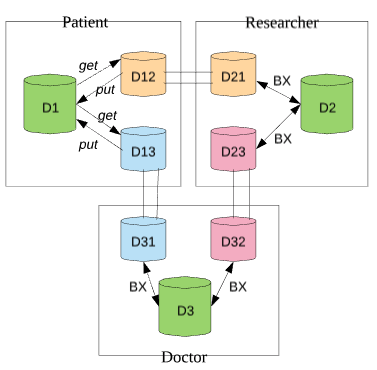
\includegraphics[width=250pt]{DBStructure.png}}
	\caption{DB architecture}
	\label{DB architecture}
\end{figure}

\begin{figure}[htbp]
	\centerline{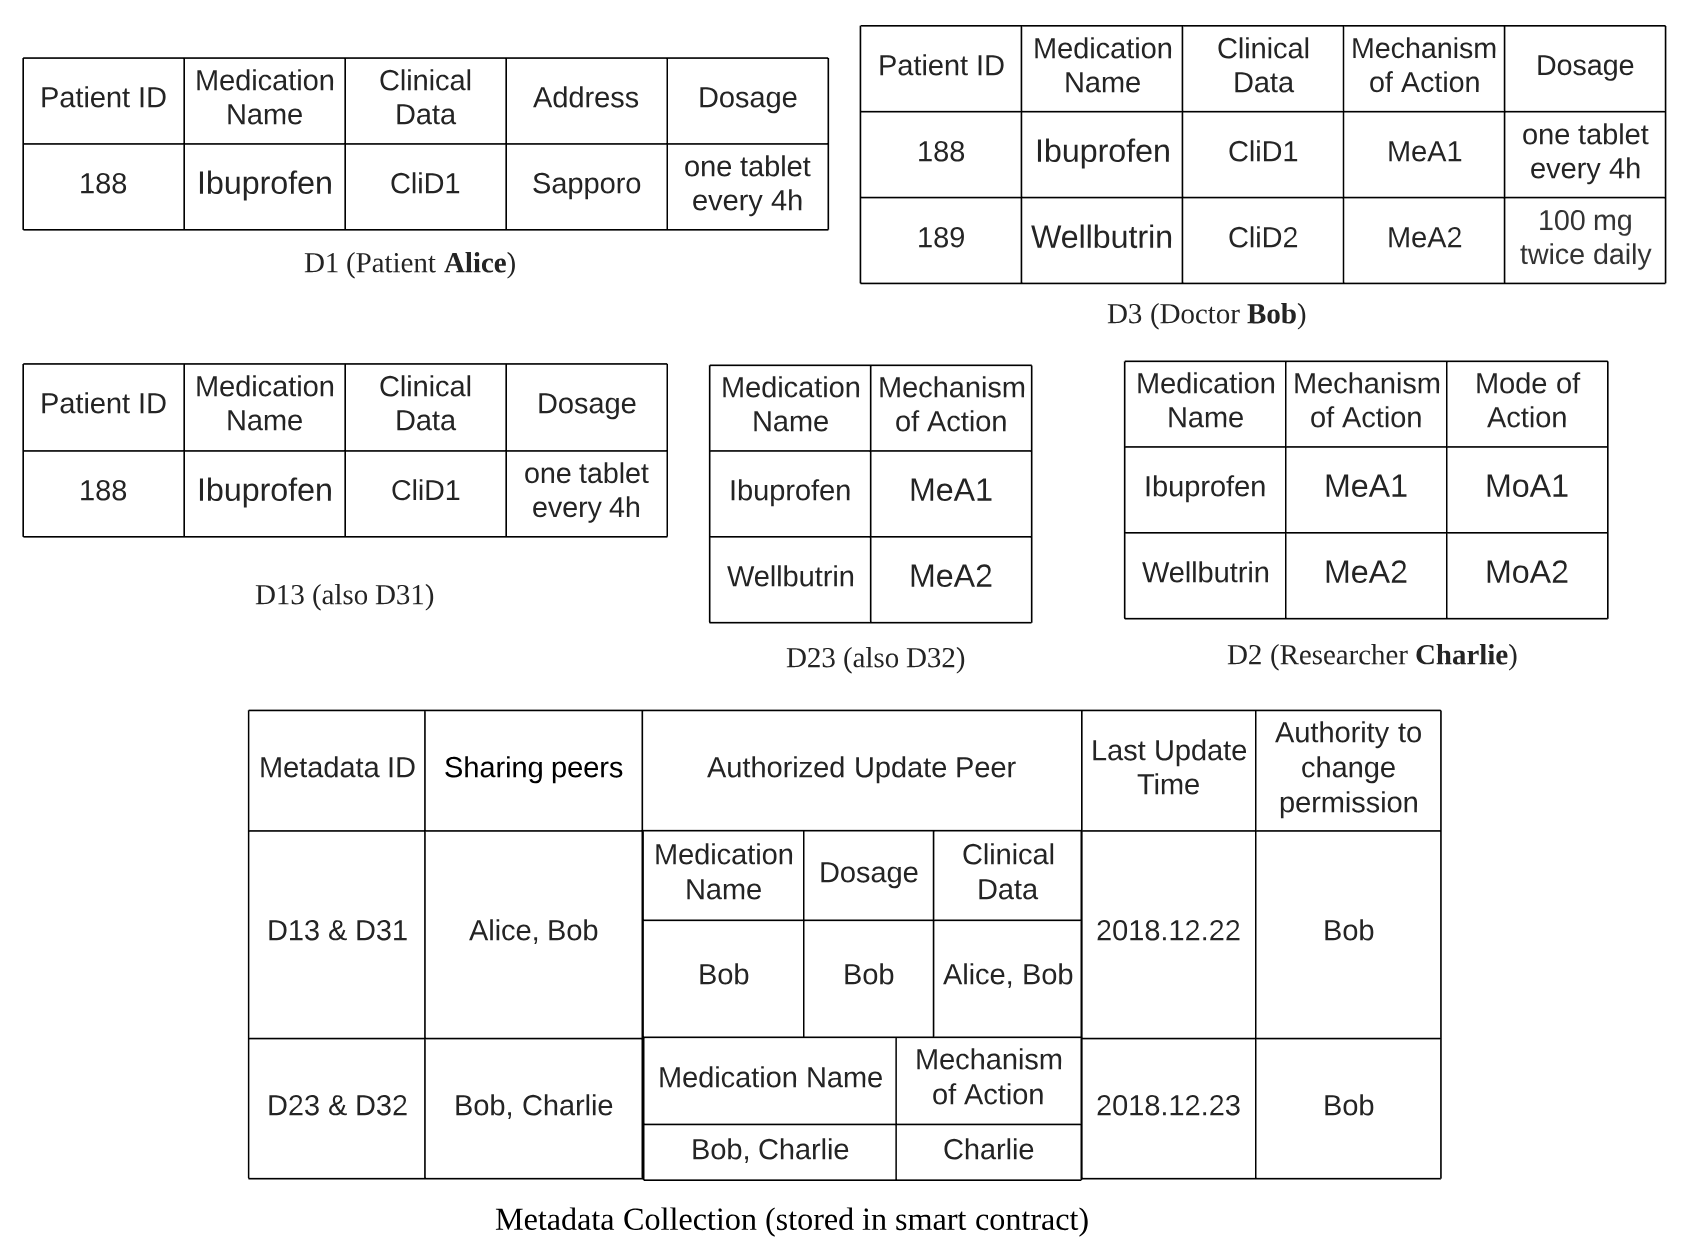
\includegraphics[width=250pt,height=220pt]{medicalData.png}}
	\caption{Data distribution}
	\label{dataRepresentation}
\end{figure}


\subsection{Permission on data management}

As shown in Fig. \ref{dataRepresentation}, the metadata collection table resides in the smart contract on blockchain. Each entry of metadata collection table corresponds to a shared table. For example, the entry for D13 or D31 declare that it is shared by Alice and Bob and Bob can update all attributes value but Alice can only change the clinical data. The ``Latest Update Time" shows when the metadata was changed most recently. Moreover, ``Authority to Change Permission" allow Bob to change other peers (here just Alice)'s authority so that Alice can update dosage by change the value for ``Dosage" attribute to ``Bob, Alice".

The metadata are created immediately once some peers wants to share data with each other. Suppose doctor Bob initiates the data sharing with patient Alice. He will deploy a smart contract on blockchain which stipulates the metadata about the shared data, such as sharing peers (i.e., Alice and Bob) and so on.  Table Metadata Collection on Fig. \ref{dataRepresentation} are built by Bob. 

Since smart contract can not be altered after it is deployed on blockchain. There are two ways to change the permission for updates to shared data:
\begin{enumerate}
	\item deploy a new contract and notify all nodes on blockchain that this new one should be used to verify authority later;
	\item update the state of variables in contract.
\end{enumerate}
We choose the latter way. In Fig. \ref{dataRepresentation}, the ability to modify the update permission are encoded in the field named as ``authority to change permission". For example, for D13 and D31, Bob can change the permission to update ``Dosage" to ``Bob, Alice" so that Patient Alice can also update the  ``Dosage" later.

\subsection{System design}
Our system consists of following components. %which can be seen from Fig. \ref{workflow}.
\begin{itemize}
	\item Front-end user interface: control the interaction between users and other components.
	
	\item Blockchain: keep a record of access and update to the shared data. Also, front-end user interfaces communicate with blockchain network via nodes. The smart contract on blockchain contains the metadata of shared medical data and maintain an update log that store historical modifications for metadata.
	
	\item Database: each user has an complete database and many data pieces shared with other users. The latter can always be reproduced from the former.
	
	\item Database manager (server) dispose the synchronization between shared data and local data in terms of consistency logic relations.

\end{itemize}

\begin{figure}[htbp]
	\centerline{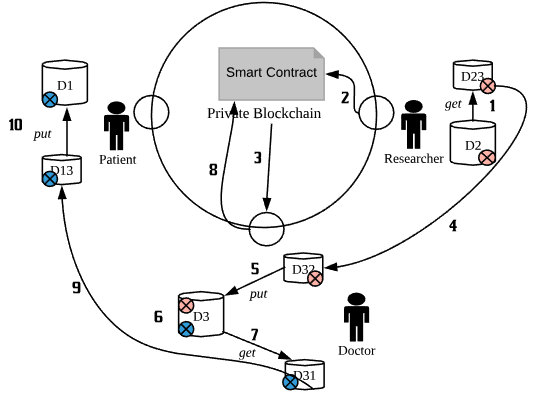
\includegraphics[width=230pt]{updateScenario.png}}
	\caption{A workflow for updating data fields of shared data}
	\label{workflow}
\end{figure}

\subsection{Case analysis}
Fig. \ref{workflow} depicts an scenario where researcher initiates the update the shared data. The numbers indicates the corresponding operations sequence. D1, D2, D3 are user's local database. D23 are identical with D32 and shared by the doctor and the researcher. D31 and D13 are same and shared by the doctor and the patient. Every shared data correspond to a BX program. For example, $BX_{23}-get$ represents the invoking on \textit{get} direction on the BX program which is used to synchronize D2 and D23. The red and blue circles with wrong sign indicate the updated places.

Let's try to describe this work flow for updating shared data. After the update on D2, the researcher wants to propagate the update to the shared data D23 so that he uses the \emph{$BX_{23}$-get} to regenerate D23 (step 1). Then he will call a smart contract via a node connected to Ethereum by sending the request for updates to the D23 (step 2). Note that the smart contract records all permission info about that D23. Only when the researcher are authorized his update are seen valid and can be propagated to D32. The smart contract will be executed until all nodes form consensus on this update request, which means researcher is permitted to update D23. Each node will conduct the smart contract locally. The entry relating D23 \& D32 of the contract are modified and doctor will receive notification that D32 need to modified (step 3). Then he will request data from the researcher by sending a message based on some encrypted communication protocol and get the newest shared data to refresh D32 (step 4). After that, doctor will use \emph{$BX_{32}$-put} to reflect the change on D32 to D3 (step 5). Since doctor shared some data (D31) with patient, he need to check whether D31 need to be reproduced (step 6). (If there is no need to reproduce, step 6 - 11 will not happen.) If yes, he will use \emph{$BX_{31}$-get} to regenerate D31 (step 7) and request smart contract for permission to update D13 (step 8). Once allowed, patient will receive the notification about the change on shared data (D31) (step 9) and ask doctor to send the updated D31. After patient get the modified D31 (step 10), he will use this to update D1 via \emph{put} (step 11).  

Step 1 - 5 achieve the propagation of updates from one peer to another. Especially, step 6 check whether the images of D32 and D32 on D3 have some dependencies. Step 7 - 11 have the same operational logic.

%
%Dependency 
%Incremental update
%Dependency graph
%
%Just send them data
%Put online; give them link
%Give data to each person
%
%Advantages of having data Locally not on server: 
%fast/easy to access
%Full control own data; change format
%exposed to others (since public available; sensitive data)
%scalability (multi access server; slow)


\section{discussion}
\label{discuss}
In this section, we add more details about our contributions. In addition, we identify some threats to our system and propose relating countermeasures.

\subsection{Detailed contributions}
\begin{itemize} %So many dots...
	\item Nodes can split total data into multiple pieces which can be shared with different nodes, which make sharing exists among only a group of nodes. So that it can avoid the interference or attack from other nodes. Meanwhile, data provider can choose what they want to share with others without exposing sensitive or private information.
	
	\item Any update on shared data can be reflected to local total database by using \emph{put}. Consistency between shared data and local total data are firmly promised by BX. 
	
	\item Permission to updates to medical data are stored in smart contracts so that blockchain can prevent operations from malicious nodes. 
	
	\item Raw medical data always stay in each peer's local database and data transfer only exist between sharing peers, which avoid data being leaked to the third party so as to keep shared data security .
	
	\item Blockchain's  consensus protocol scheme keep the shared data between sharing peers are same after updates since each peer will receive the notification from contracts and pull new shared data from other sharing peers.

	\item Any modification on shared data can be recorded on blockchain. Blockchain properties such as immutability, auditablility and transparency enable nodes to check and review update history on shared data.
	
	\item Simultaneously updates to the same shared data by multiple peers are forbidden. Smart contracts dispose the updates according to received requests in chronological order. If a transaction for updates on shared data has been included in a block, then other requests on this shared data will not be accepted, i.e., one block can contain one transaction at most on some shared data at one time. This can promise that only when all sharing peers have had newest shared data can they execute further operations.
	
	\item Each node can be a shared data provider. As referred in \cite{chung2018using},  many clinics encourage patients to collect data by themselves that are supposed to be gathered by doctors and expect to increase clinic efficiency and promote patient awareness.
	
	\item Our system can also be applied to other scenarios besides medical data sharing.
	
\end{itemize}

\subsection{Threats and countermeasures}
\subsubsection{Throughput}
We employ smart contracts to control access to shared data. As we all known that the block creation time is approximately 12 seconds on Ethereum. We argue that this time interval is acceptable since nodes may choose to collect a lot of updates then send requests to contracts. Usually it is not so urgent for a patient or doctor get the immediate updated shared data.

\subsubsection{Correctness of smart contracts }
Smart contracts might be inconsistent with specifications. We may apply some theorem prover such as Coq\cite{huet2004coq} to prove or verify the correctness of smart contracts to prevent these attacks.

\subsubsection{Public blockchain}
Once deployed to the public Ethereum blockchain, transactions relating to our systems might not be chosen into a block by miners. So a private blockchain might be a better choice for our system.

\subsubsection{Incentive}
Like in \cite{dagher2018ancile}, we don't include any incentive for mining beyond the use of our system. We presume that all nodes on the blockchain already have incentives to keep medical data from being tampered and illegal access or updates.

\section{Related work}
\label{related work}
In this section we review existing blockchain-based research on medical data sharing field and state advantages of our system compared with them.

Zyskind et al. suggested using blockchain for access control in \cite{zyskind2015decentralizing} where encrypted data reside on the third party storage. But data might be exposed by this ``trusted" third party so that data privacy are violated.

The idea of introducing Blockchain technology to healthcare was presented firstly in \cite{yue2016healthcare} where they use blockchain for data storage to guarantee medical data can not be modified by anyone. Also, they designed a Healthcare Data Gateway (HDG) to control access of the shared data. However, medical data size can become huge so that become a burden for blockchain nodes' storage since each node have the same copy of blockchain. Usually, the size of metadata is smaller than data. (It also depends on the the structure of metadata and data.) We store metadata on smart contracts so as to reduce the storage pressure for each blockchain node.
%Similarly, Patientory \cite{mcfarlane2017patientory} proposed that the medical data is stored directly on the HIPPA-compliant blockchain database.  

MedRec \cite{azaria2016medrec} choose to store raw medical data on providers' database and patients can download the data from it after authorized by smart contract on blockchain. They aimed to enable patient to engage in their healthcare. Whereas in our system, all parties, such as doctors, patients, and researchers can benefit from sharing data with others. MedRec recognized that not all provider data such as physician intellectual property can be exposed to patients \cite{us2017individuals, grossman2011clinical} so that they don't claim to manage contents automatically from physician's output. In our work, instead we allow each node share a piece of medical data not total but still keep consistency between them after the updates to the shared ones. Additionally, any modifications on data shared by two nodes will not be disclosed to the third party which keep the consistency only exists in sharing peers. Moreover, since all shared data with others can be a part of each nodes' local total databases, we can decide whether one shared data have some influence on the other shared pieces and then propagate this change to the third party.

Dubovitskaya at al. gave an architecture to mange and share medical data for cancer patient care \cite{dubovitskaya2017secure}. They stored encrypted categorized shared data on cloud and relating metadata in blockchain and implemented the prototype on Hyperledger\cite{hyperledger2017hyperledger}. The access control policy are defined in the chaincode Logic by patients. Whereas we think that each data provider not just patients can use smart contracts to encode the control policy when they deploy them to Ethereum. 

Notably, previous three works and others \cite{liu2018bpds,xia2017bbds,amofa2018blockchain,dagher2018ancile,fan2018medblock} mostly targeted to the access problem on shared data but did not pay much attention to updates on the them. Additionally, they presumed that different parties can share the same data. Unlike them, we aims to solve the updates issues on the shared data and allow one party can split total data into multiple pieces (i.e, views) which are shared with different parties but still keep consistency between source and views.

%Distributed Authorized Medical Data Management
\section{Conclusion}
\label{conclude}

Medical data sharing are necessary and important, which allow stakeholders on medical scenarios to contribute their knowledge to better the medical treatment. Users may have different interest on the same complete medical record. Some peers might update some values of fields in the existing data. This updates need to be propagated to sharing peers. Our architecture divides a record into pieces that shared with different users separately, which can protect data privacy by limiting essential data between two peers and reduce the unrelated data interference. Any updates on data pieces can be synchronized to complete records by bidirectional transformations. Moreover, based on smart contracts on blockchain, we can promise that only authorized users can update the existing shared data and only when all peers have updated to the newest data contents they can continue the operations on shared data.   

We are still developing the prototype to implement our idea.
In the future, we will use the real patient data to do experiment but use some de-identification technology to protect patient data from being exposed. 

\section*{Acknowledgment}
The authors would like to thank all PRL lab members for their helpful advice in the paper draft.  Thanks Hsiang-Shang Ko for revising the BX parts and providing valuable suggestions to our work. Thanks Van-Dang Tran's help on building the initial data distribution idea sketch. This work is partially supported by the Japan Society for the Promotion of Science (JSPS) Grant-in-Aid for Scientific Research (S) No. 17H06099 and Scientific Research (A) No. 18H04093.

\bibliographystyle{IEEEtran}
\bibliography{ref}

\end{document}
